\subsection{Travail sur frochet/quiceh}

\subsubsection{Implémentation de la FFI}

Le code de frochet/quiceh est une bibliothèque, c'est-à-dire que ce code seul ne fait rien, il fournit seulement des fonctionnalités qui peuvent être utilisées dans d'autres programmes.
Un de ces programmes est cURL. cURL est un logiciel permettant d'effectuer des requêtes HTTP en ligne de commande. C'est un logiciel très important pour les développeurs sous Linux, car il est utilisé par des milliers d'autres logiciels.
cURL utilise cloudflare/quiche comme base pour effectuer des requêtes HTTP/3. Or Daniel Stenberg, le développeur principal de cURL se plaint régulièrement des performances d'HTTP/3\up{\cite{stenberg-complaining}}. Cela fait de cURL un choix parfait pour expérimenter le remplacement de cloudflare/quiche par frochet/quiceh et mesurer le gain de performances.

cURL est écrit en langage C tandis que frochet/quiceh est écrit en Rust, il a donc fallu écrire une FFI dans frochet/quiceh pour fournir à cURL une version C des fonctions de Quiceh.
On trouve près de 3500 fonctions dans le code de Quiceh; fort heureusement il n'est pas nécessaire d'écrire une interface C pour chaque fonction de Quiceh. Seules les fonctions utilisées par les programmes externes comme cURL doivent bénéficier d'une FFI, la plupart des fonctions sont des fonctions internes à Quiceh qui n'ont pas besoin d'interface C.
De plus, comme frochet/quiceh est dérivé du code de cloudflare/quiche, la plupart de la FFI était déjà écrite, il fallait écrire la FFI pour toutes les nouvelles fonctions de QUIC VReverso qui fonctionnent sans copie.

\begin{figure}[H]
    \centering
    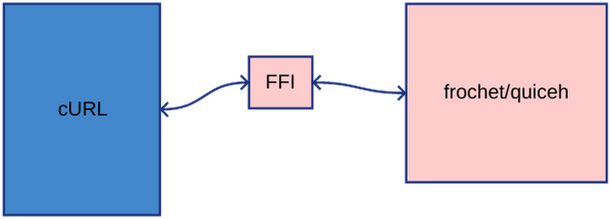
\includegraphics[height=0.15\textheight]{figures/curl_ffi_quiceh.png}
    \caption{La FFI est un morceau de code entre 2 projets écrits dans des langages différents}
\end{figure}

La FFI doit être écrite en langage Rust, n'ayant jamais fait de Rust auparavant, j'ai dû me former sur le langage et la syntaxe de ses FFI. Une fois ceci fait, j'ai pu rapidement écrire la dizaine de fonctions requises par cURL, en les testant non pas sur cURL mais sur un client HTTP très minimaliste en C que j'ai conçu pour l'occasion.

\subsubsection{Portage de frochet/quiceh dans cURL}

Une fois les fonctions de la FFI écrites dans frochet/quiceh, il fallait modifier le code de cURL pour les utiliser.
Malheureusement, cela ne pouvait se résumer à remplacer les fonctions de cloudflare/quiche par celles de frochet/quiceh. Le code de cURL n'était pas du tout conçu pour utiliser les interfaces zéro copie.
cURL copie tous les buffers qu'il reçoit et qu'il doit envoyer dans une queue interne. Si l'on utilise les fonctions de frochet/quiceh dans ce contexte, les données vont se retrouver corrompues car les buffers sont réutilisés.
On peut contourner le problème en copiant systématiquement les buffers dans de nouveaux avant de les ajouter à la queue, mais si l'on fait ça on déplace la copie depuis Quiche vers cURL au lieu de vraiment retirer cette copie.

\begin{figure}[H]
    \centering
    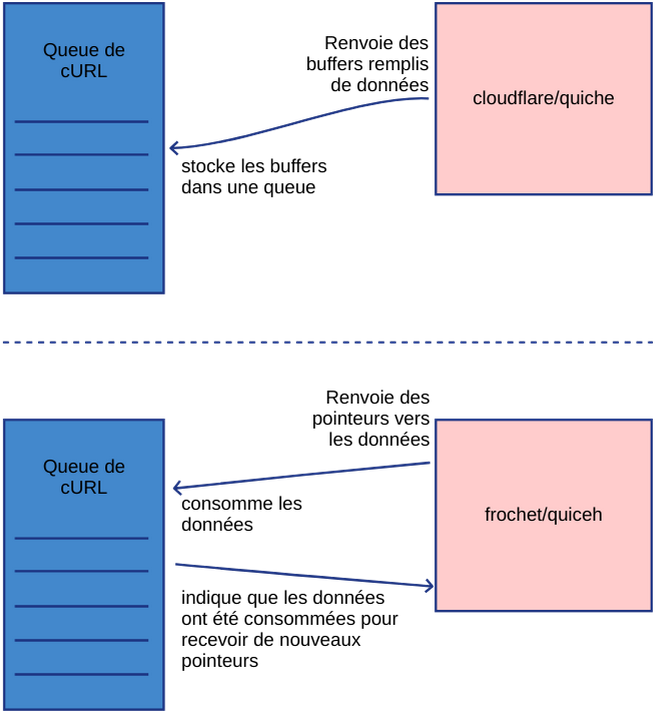
\includegraphics[height=0.37\textheight]{figures/curl_queue.png}
    \caption{\small{La différence de fonctionnement entre cloudflare/quiche et frochet/quiceh rend la queue de cURL inadaptée, car il faudrait copier les données pour les consommer.}}
\end{figure}

Pour mesurer un vrai gain de performance, la seule solution était de trouver un moyen de contourner la queue de cURL lorsqu'on utilise QUIC VReverso. A noter qu'il faut aussi garder l'ancienne queue et l'ancien fonctionnement pour le cas où le pair négocie QUIC V1 plutôt que QUIC VReverso.

\newpage

\subsection{Deuxième sous partie}

\subsubsection{A}

    \lipsum[1-2]

\subsubsection{B}

    \lipsum[1-2]